% !TEX program=luatex
\documentclass[11pt,a4paper]{article}
\usepackage{luatexja-fontspec}
\setmainjfont{FandolSong}
\usepackage{amsmath}
\usepackage{amsthm}
\usepackage{amssymb}
\usepackage{amsfonts}
\usepackage{enumerate}
\usepackage{graphicx} 
\usepackage[colorlinks]{hyperref}
\usepackage{tikz-cd}
\usepackage{geometry}
\geometry{left=2cm,right=1cm, top=3cm,bottom=2cm}
\usepackage{simplewick}
\theoremstyle{definition}
\newtheorem{secdefn}{Definition}[subsection]
\newtheorem{exer}{Exercies}[subsection]
\newcommand*{\qeds}{\hfill\ensuremath{\clubsuit}}
\DeclareMathOperator{\res}{Res}
\begin{document}
\noindent
{\LARGE\underline{\textbf{2d CFT}}}\\
{\hfill\large  \underline{\textbf{邹海涛}} \\
	\hfill ID: 17210180015}\\
%\normalsize ECE 100-003 \hfill Teammates: Student1, Student2 \\
%TA: Adam Sumner \hfill Due Date: XX/XX/XX
\section*{Week 1}
\begin{exer}
	The first order transitions and second order transitions show in the diagram
	\begin{figure}[h]
		\centering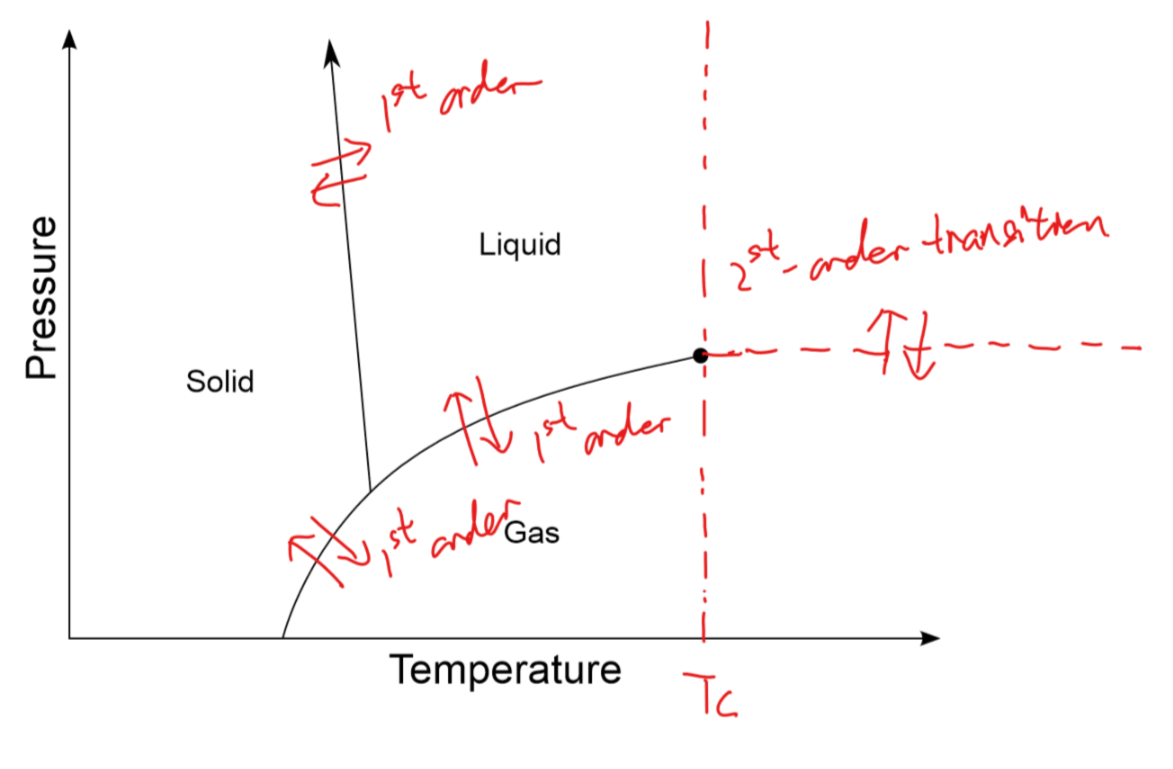
\includegraphics[scale=0.5]{PIC/hw1.png}
	\end{figure}
\end{exer}
\begin{exer}
	By the homogeneous relation
\[
f(t,h)= b^{-d}f(b^{y_t} t, b^{y_h} h)
\]
we have 
\[
f(t,h)= t^{\frac{d}{y_t}}g(\alpha)
\]
where $g(\alpha) = f(1,\alpha)$ and $\alpha = t^{-\frac{y_h}{y_t}}h$. It is easy to see that $\alpha$ is invariance under scaling transformation $x \to x/b$.
Hence we have 
\[
\begin{aligned}
&C(t,0) = -T \frac{\partial ^2 f}{\partial T ^2}\big|_{h=0} = - \frac{1}{T_c} t^{\frac{d}{y_t}-2}g''(0) \\
& M(t,0) = -\frac{\partial f}{\partial B}\big|_{h=0} =t^{\frac{d-y_h}{y_t}}g'(0)\\
& \chi(t,0) = \frac{\partial^2 f}{\partial B^2}\big|_{h=0} = t^{(d-2y_h)/y_t} g''(0)\\
\end{aligned}
\]
As function with single variable $h$, $\lim_{t \to 0}  M(t,h) \sim h^{\frac{1}{\delta}}$, which implies that $g'(\alpha) \sim \alpha^{\frac{1}{\delta}}$ since $\alpha$ is linear function of $h$. Hence we have 
\[
\lim_{t \to 0} M = \lim_{t \to 0} t^{(d-y_n - \frac{y_n}{\delta})}h ^{1/\delta}
\]
since it is non-zero, we have $d- y_n - y_n \frac{1}{\delta}=0$. Hence we have 
\[
\delta = \frac{y_h}{d-y_h}
\]	
\end{exer}
\begin{exer}
	We have following relation
	\begin{equation}\label{eq1}
	G_{\sigma}(\mathbf{r};t,h) = t^{-2x_{\sigma}}G_\sigma (\frac{\mathbf{r}}{b};b^{y_t}t,b^{y_h}h)
	\end{equation}
	Let $h=0, K= b^{y_t}t$,	
	\[
	G_{\sigma}(\mathbf{r};t,0) = t^{2x_{\sigma}/y_{t}}G_\sigma (\frac{\mathbf{r}}{K t^{-1/y_{t}}};K,0)
	\]
	Since $ G_{\sigma}(\mathbf{r}) \sim r^{-\tau} e^{-\frac{r}{\xi}}$, we have $\xi \sim t^{-1/y_t}$. It implies $\nu = 1/y_t$. With relation \ref{eq1}, we have 
	\[
	\chi(t,h)= \frac{1}{T} \int d^d \mathbf{r} G_\sigma (\mathbf{r};t,h)= t^{d-2x_\sigma} \chi (b^{y_t}t, b^{y_h}h)
	\]
	So $\gamma = (d-2x_\sigma)/y_t$. But we have $\eta = 2 x_\sigma +2 -d$ for finite limit of $G(r)$ when $t \to 0$ and $h=0$. Therefore, we get
	\[
	\gamma = \nu(2-\eta)
	\]With scaling relations
	\[
	\begin{aligned}
	\alpha + 2 \beta + \gamma =2\\
	\alpha + \beta (1+\delta) =2\\
	\end{aligned}
	\]
	and $\alpha = 2 -d \nu$, we have
	\[
	\begin{aligned}
	\beta &= \frac{d\nu -2\nu + \nu \eta}{2}\\
	\delta &= \frac{d-\eta +2}{d+\eta -2}\\
	\end{aligned}
	\]
	\end{exer}
\begin{exer}
	By listed commutation relations, we have, for $r, s > 0$,
	\[
	\begin{aligned}
	&[D, J_{rs}]= [D, L_{rs}] = \frac{i}{2} [D, [K_r, P_s]]\\
	 & =-\frac{i}{2}\big([P_s,[D,K_r]]+ [K_r,[P_s,D]]\big)\\
	 & =\frac{1}{2}[P_s, K_r] -\frac{1}{2}[K_r, P_s]\\
	 &=0
	\end{aligned}
	\]
	For $r=-1,s=0$, $[D,J_{rs}]= [D,D]=0$. For $r=-1, s\neq 0$, $[D,J_{-1,s}]=[D,\frac{1}{2}(P_s - K_s)]= \frac{i}{2}(P_s +K_s)$. For $r=0$, $[D, J_{0s}] = \frac{i}{2}(P_s - K_s)$. Hence (2,25) is satisfied when $(m,n)=(-1,0)$.
	
	If $(m,n)=(-1,n)$, then we have 
	\[
	[J_{mn},J_{rs}] = \frac{1}{2}[P_n, J_{rs}] -\frac{1	}{2} [K_n, J_{rs}]
	\]
	With listed commutation relations, we can easily check it coincides with (2,25) respectively. Similarly check in the case of $(m,n)= (0,n)$. 
\end{exer}
\newpage
\noindent
{\LARGE\underline{\textbf{2d CFT}}}\\
{\hfill\large  \underline{\textbf{邹海涛}} \\
	\hfill ID: 17210180015}\\
\section{$SL_2(\mathbb{C})$}
\begin{exer}
	We have $\det X = t^2-(x^2+y^2+z^2)$. Since points in $\mathbb{R}^{1,3}$ can be written with Pauli matrix as base. Elements in $SO(1,3)$ can be viewed as action on $M_2(\mathbb{C})$ with form $P \mapsto PXP^*$, which preserve det of $X$.
	We have exact sequence of groups as follows:
	\[\begin{tikzcd}
		0 \ar[r] &\mathbb{Z}_2 \ar[r] &SL_2(\mathbb{C}) \ar[r,"sp"]&SO(1,3) \ar[r]&1 
	\end{tikzcd}\]
	where $\text{sp}$ is map $P \mapsto (X \mapsto PXP^*)$. Since for $P \in SL_2(\mathbb{C})$, $\det(PXP*) = \det(X) = t^2-(x^2+y^2+z^2)$, $sp$ is well-defined. Hence $SO(1,3) \cong SL_2(\mathbb{C})/\mathbb{Z}_2$.
\end{exer}
\begin{exer}
	\begin{itemize}
		\item \[
		z \mapsto \frac{(z_2 -z_3)(z-z_1)}{(z_2-z_1)(z-z_3)}
		\]
		\item We have
		\[
		\begin{aligned}
		(w_1 -w_3)=&\frac{(az_1+b)(cz_3+d)-(az_2 +b)(cz_4+d)}{(cz_1+d)(cz_3+d)}\\
		=&\frac{z_1-z_3}{(cz_1+d)(cz_3+d)}
		\end{aligned}
		\]
		Hence we have $[z_1,z_2,z_3,z_4]=[w_1,w_2,w_3,w_4]$.
	\end{itemize}
\end{exer}
\section{Three-point function}
\begin{exer}
	Let $\langle\phi_1(z_1)\phi_2(z_2)\phi_3(z_3)\rangle =f(z_{12},z_{23},z_{13})$. Under scalar transformation $z_i \mapsto \lambda z_i$, we have
	\[
	f(z_{12},z_{23},z_{13})=\lambda^{h_1+h_2+h_3}f(\lambda z_{12},\lambda z_{23},\lambda z_{13})
	\]
	Therefore, $f$ is with form
	\[
	f(z_{12},z_{23},z_{13})=\frac{C_{123}}{z_{12}^a z_{23}^b z_{13}^c}
	\]
	where $a+b+c = h_1 +h_2 +h_3$.
	Then under comformal transformation $z_i \mapsto \frac{1}{z_i}$, we have
	\[
	{z_1}^{-2h_1}{z_2}^{-2h_2}{z_3}^{-2h_3} \frac{(z_1z_2)^a(z_2 z_3)^b(z_1z_3)^c}{z_{12}^a z_{23}^b z_{13}^c}= \frac{1}{z_{12}^a z_{23}^b z_{13}^c}
	\]
	Hence $a= h_1 +h_2 -h_3, b=h_2 + h_3 -h_1, c= h_1 +h_3 - h_2$.
\end{exer}
\section{Energy-momentum tensor}
\begin{exer}
	\begin{itemize}
		\item \[
		T^{\mu \nu} = -\eta^{\mu \nu}\partial_{k}\varphi \partial^{k}\varphi + 2 \partial^{\mu}\varphi \partial^{\nu}\varphi
		\]
		\item We have
		\[
			\delta \sqrt{g}= -\frac{1}{2}\sqrt{g} g_{\mu\nu} \delta g^{\mu\nu}
		\]
		Therefore,
		\[
		\begin{aligned}
		\tilde{T}^{\mu\nu} &=\frac{2}{\sqrt{g}}\frac{\delta S}{\delta g^{\mu\nu}}\\
		&=\frac{1}{2} (-\delta_{\mu\nu}+2) \partial_{\mu} \varphi \partial_{\nu}\varphi
		\end{aligned}
		\]
	\end{itemize}
\end{exer}
\newpage
\noindent
{\LARGE\underline{\textbf{2d CFT}}}\\
{\hfill\large  \underline{\textbf{邹海涛}} \\
	\hfill ID: 17210180015}\\
\section{Derivations}
	\subsection{Energy-momentum tensor in complex coordinate}
	Since 
	\[
	\begin{aligned}
	&\partial_0 \Phi = \partial_z \Phi + \partial_{\bar{z}}\Phi\\&\partial_1 \Phi = i\partial_z \Phi - i \partial_{\bar{z}}\Phi
	\end{aligned}
	\]
	we have \[
	\begin{aligned}
	&\partial_z \Phi =\frac{1}{2} \partial_0 \Phi - \frac{i}{2} \partial_1 \Phi\\& \partial_{\bar{z}} \Phi = \frac{1}{2} \partial_0 \Phi+ \frac{i}{2} \partial_1 \Phi
	\end{aligned}
	\] 
	Also, since there are metric tensors in complex coordinates
	\[
	\begin{aligned}
	g^{\alpha \beta}= \begin{pmatrix}
	0&2 \\
	2&0\\
	\end{pmatrix}& &g_{\alpha \beta}\begin{pmatrix}
	0& \frac{1}{2}\\
	\frac{1}{2}& 0\\
	\end{pmatrix}
	\end{aligned}
	\],
	we have $\partial^z \Phi = 2 \partial_{\bar{z}}$ and $\partial^{\bar{z}} \Phi = 2\partial_{\bar{z}} \Phi$. Therefore, from definition of energy-momentum tensor
	\[T_{\alpha \beta}= - g_{\alpha \beta} \mathcal{L}+ \frac{\partial \mathcal{L}}{\partial (\partial^\alpha \Phi)} \partial_\beta \Phi
	\] we get expression of them in complex coordinates
	\[
	\begin{aligned}
	&T_{zz} = \frac{1}{4}\big( \frac{\partial \mathcal{L}}{\partial_0 \Phi} \partial_0 \Phi - i \frac{\partial}{\partial_1 \Phi} \partial_0 \Phi - i \frac{\partial \mathcal{L}}{\partial_0 \Phi} \partial_1 \Phi - \frac{\partial \mathcal{L}}{\partial_1 \Phi} \partial_1 \Phi\big)\\
	&T_{\bar{z}\bar{z}} = \frac{1}{4}\big( \frac{\partial \mathcal{L}}{\partial_0 \Phi} \partial_0 \Phi + i \frac{\partial}{\partial_1 \Phi} \partial_0 \Phi + i \frac{\partial \mathcal{L}}{\partial_0 \Phi} \partial_1 \Phi - \frac{\partial \mathcal{L}}{\partial_1 \Phi} \partial_1 \Phi \big)\\
	&T_{z \bar{z}} = - \frac{1}{2} \mathcal{L} + \frac{1}{4} \big( \frac{\partial \mathcal{L}}{\partial_0 \Phi} \partial_0 \Phi - i \frac{\partial}{\partial_1 \Phi} \partial_0 \Phi + i \frac{\partial \mathcal{L}}{\partial_0 \Phi} \partial_1 \Phi + \frac{\partial \mathcal{L}}{\partial_1 \Phi} \partial_1 \Phi\big)\\
	&T_{z \bar{z}} = - \frac{1}{2} \mathcal{L} + \frac{1}{4} \big( \frac{\partial \mathcal{L}}{\partial_0 \Phi} \partial_0 \Phi + i \frac{\partial}{\partial_1 \Phi} \partial_0 \Phi - i \frac{\partial \mathcal{L}}{\partial_0 \Phi} \partial_1 \Phi + \frac{\partial \mathcal{L}}{\partial_1 \Phi} \partial_1 \Phi\big)\\
	\end{aligned}
	\]
	Hence 
	\[
	\begin{aligned}
	&T_{zz} = \frac{1}{4} (T_{00} - 2i T_{10} - T_{11})\\
	&T_{\bar{z} \bar{z}} = \frac{1}{4} (T_{00} +2i T_{10} - T_{11})\\
	&T_{z\bar{z}} =T_{\bar{z}z}= \frac{1}{4} (T_{00} + T_{11})\\
	\end{aligned}
	\]
\subsection{Schwarzian derivative}
\[
\tilde{T}(z+\epsilon(z)) = (1+ \partial_z \epsilon(z))^{-2}\Big[T(z)- \frac{c}{12}\big(\frac{\partial_z^3\epsilon(z)}{1+\partial_z\epsilon(z)}-\frac{2}{3} \frac{\partial_z^2 \epsilon(z)}{1+\partial_z \epsilon(z)}\big)\Big]
\]
Since 
\[
\frac{1}{1+\partial_z \epsilon(z)} = 1- \partial_z \epsilon(z) + (\partial_z \epsilon)^2 + \cdots
\]
we have 
\[
\begin{aligned}
\tilde{T}(z+ \epsilon(z)) &\approx T(z)(1-2\partial_z \epsilon(z)) - \frac{c}{12} (\partial^3_z \epsilon(z) - \frac{2}{3} \partial^2_z \epsilon(z))\\
& \approx T(z) - 2 \partial_z\epsilon(z) T(z) - \frac{c}{12}\partial^3_z\epsilon(z)
\end{aligned}
\]
Hence
\[
\tilde{T}(z+ \epsilon(z)) - \big[\epsilon(z)\partial_z T(z) +T(Z)\big] \approx -\frac{c}{12} \partial^3_z\epsilon(z) - 2 \partial_z\epsilon(z)T(z) -\epsilon(z)\partial_z T(z) 
\]
It implies that $\delta_\epsilon(T(z)) = -\frac{c}{12} \partial^3_z\epsilon(z) - 2 \partial_z\epsilon(z)T(z) -\epsilon(z)\partial_z T(z) $.
\subsection{Virasoro algebra}
The Larrent expansion of $z^{n+1}$ around $\omega$ is 
\[
z^{n+1}= (z- \omega)^{n+1} + \binom{n+1}{1} \omega (z-\omega)^n + \cdots + \binom{n+1}{i}\omega^i (z-\omega)^{n+1 -i} +\cdots + \omega^{n+1}
\]
 Hence we have following residues:
 \[
 \begin{aligned}
 &\res_{\omega} \frac{z^{n+1}}{(z-\omega)^4}= 2 \pi i \frac{(n+1)n(n-1)}{6} \omega^{n-2}\\ 
&\res_{\omega} \frac{z^{n+1}}{(z-\omega)^2}= 2 \pi i (n+1) \omega^n\\
&\res_{\omega} \frac{z^{n+1}}{z-\omega}= 2 \pi i \omega^{n+1}
 \end{aligned}
 \]
  Hence we have 
  \[
  \begin{aligned}
  &[L_n, L_m] = \frac{1}{(2 \pi i )^2} \oint_0 d \omega\ \omega^{m+1} \oint_\omega dz\ z^{n+1} \big(\frac{c}{2(z-\omega)^4} + \frac{2T(\omega)}{(z-\omega)^2} + \frac{\partial_\omega T(\omega)}{(z-\omega)} + \text{regular part}\big)\\
  &= \frac{1}{2 \pi i} \oint_0 d\omega\ \omega^{m+1} \big( \frac{c}{12}(n+1)n(n-1) \omega^{n-2} + 2(n+1) \omega ^n T(\omega) + \omega^{n+1} \partial_{\omega} T(\omega) \big)&\\
 &= \frac{1}{2 \pi i} \Big\{\oint_0 d\omega\ \Big( \frac{c(n+1) n(n-1)}{12} \omega^{m+n-1} )\Big) - (m-n) \oint_0 d\omega \omega^{m+n +1 } T(\omega) \Big\}&\\
 &= \frac{c}{12} n (n^2-1) \delta_{n+m,0} - (m-n) L_{n+m}
  \end{aligned}
  \]
 \subsection{Commutation relations in free boson}
 We have 
 \[
 \varphi = \varphi_0 + \frac{4\pi}{l} \pi t + i \sum_{n \neq 0} \frac{1}{n} \Big( a_n e^{-2 \pi in (t-x)/l} + \bar{a}_n e^{-2 \pi n (t+x)/l}\Big)
 \]
 on cylinder. 
 \[
 \Pi = \frac{\pi_0}{l}+ \frac{1}{2l} \sum_{n \neq 0} \Big(a_n e^{-2\pi i n (t-x)/l} + \bar{a}_n e^{-2 \pi i n (t+x) /l}\Big)
 \]
  With $[\Pi, \Pi]=0$, we can get $[\pi_0, a_n] =0$ and $[\pi_0, \bar{a}_n]=0$. Furthermore, since $[\varphi, \varphi]=0$, we have $[\varphi_0, a_n]= [\varphi_0 ,\bar{a}_n]=0$.
  \[
  \begin{aligned}
  &i \delta(x-y)=[\varphi(x,t), \Pi(y,t)]&= \frac{1}{l} [\varphi_0, \pi_0] + \frac{i}{2l} \sum_{n \neq 0, m \neq 0} \frac{1}{n}\Big([a_n, \bar{a}_m] \exp(-2 \pi i [(n+m)t -nx+my]/l)\\
  && + [\bar{a}_n, a_m] \exp(-2\pi i [(n+m)t +nx -my]/l) \\
  && + [a_n, a_m] \exp(-2\pi i [(n+m)t -nx -my]/l) \\
  && + [\bar{a}_n, \bar{a}_m] \exp(-2\pi i [(n+m)t +nx+my]/l)\Big)\\
  \end{aligned}
  \]
  Since $t$ can be arbitrary, $[a_n, \bar{a}_m] = [\bar{a}_n, a_m] =0$ when $n+m \neq 0$. Then let $t=0$, we get\[
  \begin{aligned}
  i \delta(x-y)&=[\varphi(x,0), \Pi(y,0)] \\
  &= \frac{1}{l}[\varphi_0, \pi_0] + \frac{i}{2l} \sum_{n \neq 0}\frac{1}{n} \Big([a_n, \bar{a}_{-n}] e^{- 2 \pi i (-nx -ny)/l} + [\bar{a}_n, a_{-n}] e^{-2 \pi i (nx+ny)/l} + \text{other terms}\Big)\\
   & = \frac{1}{l}[\varphi_0, \pi_0] + \frac{i}{l} \sum_{n \neq 0} \Big( \frac{2[a_n, \bar{a}_{-n}]}{n}  \Big)e^{2 \pi i(n(x+y))/l} + \text{other terms}
  \end{aligned}
  \]
  Since $e^{2 \pi i (n(x+y))/l}$ is independent of $x-y$, then its coefficient is zero. Hence $[a_n, \bar{a}_{-n}]=0$.
  Take integral of both left and right side, we can get $[\varphi_0, \pi_0] = i$ and $[a_n, a_{-n}] = [\bar{a}_n, \bar{a}_{-n}] = 1$.
 \subsection{Hamitonian in free boson}
 \subsection{Action of free fermion}
 \[
 S = \frac{1}{4\pi} \int d^2 x \psi^\dagger \gamma^0(\gamma^0 \partial_0 \psi + \gamma^1 \partial_1 \psi)
 \]
 But
 \[
 \gamma^0(\gamma^0 + \gamma^1) \psi = \begin{pmatrix}
 \partial_0 + i \partial_1& 0 \\
 0 & \partial_0 - i \partial_1\\
 \end{pmatrix} \psi
 \]
 Write $\psi$ as $\begin{pmatrix}
 \varphi\\ \bar{\varphi}
 \end{pmatrix}$, then we have $$ \gamma^0(\gamma^0 + \gamma^1) \psi = \begin{pmatrix}
 2\partial_{\bar{z}} \varphi\\ 2 \partial_{z} \bar{\varphi}
 \end{pmatrix}$$
 Hence 
 \[
	S = \frac{1}{2\pi} \int d^2 x (\bar{\varphi} \partial_{z} \bar{\varphi} +  \varphi \partial_{\bar{z}} \varphi)
 \]
 \subsection{$TT$ OPE in free fermion}
By derivative, we get 
\[
\begin{aligned}
\langle \psi (z), \partial_\omega \psi(\omega) \rangle \sim \frac{1}{(z-\omega)^2}& \\
 \langle \partial_z \psi , \partial_\omega \psi \rangle \sim \frac{-2}{(z-\omega)^3}&\\
\end{aligned}
\]
Hence 
\[
\begin{aligned}
T(z) \partial_\omega \psi(\omega) & = \frac{1}{2} : \psi(z) \partial_z \psi(z): \partial_\omega \psi(\omega)\\
& \sim -\frac{\psi(\omega)}{(z-\omega)^3} - \frac{1}{2} \frac{\partial_\omega \psi (\omega)}{(z-\omega)^2}
\end{aligned}
\]
and 
\[
\begin{aligned}
T(z)T(\omega) &= \frac{1}{4} : \psi(z) \partial_z \psi(z) :: \psi(\omega) \partial_\omega \psi(\omega)\\
& \sim \frac{1}{4} \big\{ - \frac{:\partial_z \psi(z) \partial_\omega \psi(\omega)}{z-\omega} + \frac{2: \psi(z) \psi(\omega):}{(z-\omega)^3} - \frac{: \psi(z) \partial_\omega \psi(\omega) + \partial_z \psi(z) \psi(\omega):}{(z-\omega)^2} + \frac{1}{(z-\omega)^4} \big\}\\
&\sim \frac{1}{4} \big\{\frac{2 \partial_\omega T(\omega)}{z-\omega} + \frac{4T(\omega)}{(z-\omega)^2} + \frac{1}{(z-\omega)^4}  \big\}
\end{aligned}
\]
\section{Vertex operator and OPE}
If we write $\varphi(z,\bar{z})$ into laurent series since $\varphi$ is free boson, then we can find $\exp(ik \varphi)$ is product of infinite exponential components which are commutative. Hence the normal ordering has taylor expansion form
\[
:\exp(ik \varphi(z,\bar{z})): = \sum_{n=0}^{\infty} \frac{(ik)^n}{n!}: \varphi(z,\bar{z})^n:
\]
To justify that $:\exp(ik \varphi):$ is primary field, we calculate its OPE
\[
\begin{aligned}
T(z):\exp{ik \varphi(\omega,\bar{\omega})}:& = - \frac{1}{2} \sum_{n=0}^{\infty} : \partial \varphi(z) \partial \varphi(z) :: \varphi(\omega, \bar{\omega})^n\\
&\sim - \sum_{n=1}^{\infty} \frac{(ik)^n}{n!} n : \partial \varphi(z) \overbrace{\partial \varphi(z) \varphi(\omega,\bar{\omega})} \varphi(\omega,\bar{\omega})^{n-1}:\\
&- \frac{1}{2}\sum_{n=2}^{\infty} \frac{(ik)^n}{n!} n(n-1) : \overbrace{\partial \varphi(z) \overbrace{\partial \varphi(z) \varphi(\omega, \bar{\omega})} \varphi(\omega,\bar{\omega})} \varphi(\omega,\bar{\omega})^{n-2}:\\
&\sim \frac{ik \partial_\omega \varphi(\omega)}{z-\omega}:\exp(ik\varphi): +\frac{k^2}{2(z-\omega)^2} :\exp(ik\varphi):\\
\end{aligned}
\]
This form implies that $:\exp(ik\varphi):$ is primary field with conformal dimension $\frac{k^2}{2}$.
\section{$bc$ ghost system}
 \[
 \begin{aligned}
 T(z) b(\omega) & = (-2: b(z) \partial c(z): + :c(z) \partial b(z):) b(\omega)\\
 & 2 \frac{b(z)}{(z-\omega)^2} - \frac{\partial_z b(z)}{z-\omega}\\
 \end{aligned}
 \]
 Take Taylor expansion of $b(z)$ and $\partial_z b(z)$ around $\omega$, we have
 \[
 T(z)b(w) \sim 2\frac{b(\omega)}{(z-\omega)^2} + \frac{\partial_\omega b(\omega)}{z-\omega}
 \]
 Hence the conformal dimension of $b$ is $2$.
 
 Similarly, we have
 \[
 \begin{aligned}
 T(z) c(\omega) & = (-2: b(z) \partial c(z): + :c(z) \partial b(z):) c(\omega)\\
 & \sim - \frac{c(z)}{(z-\omega)^2} + 2\frac{\partial_z c(z)}{z-\omega}\\
 & \sim -\frac{c(\omega)}{(z-\omega)^2} + \frac{\partial_\omega c(\omega)}{z-\omega}
 \end{aligned}
 \]
Hence conformal dimension of $c$ is $-1$.
 \[
 \begin{aligned}
 T(z)T(\omega)&= 4 :b(z) \partial c(\omega): : b(\omega) \partial c(\omega):\\
 & - 2: c(z) \partial b(z) :: b(\omega) \partial c(\omega): - 2: b(z) \partial c(z):: c(\omega) \partial b(\omega):\\
 & + c(z)\partial b(z) :: c(\omega) \partial b(\omega):\\
 \end{aligned}
 \]
 We will calculate it term by term
 \[
 \begin{aligned}
& 4:b(z) \partial c(z):: b(\omega) \partial c(\omega):\\
&\sim 4 \Big(: \overbrace{b(z) \partial c(z)b(\omega) \partial c(\omega)}: + b(z)  \overbrace{\partial c(z)  b(\omega)} \partial c(\omega)+: \overbrace{b(z) \overbrace{\partial c(z) b(\omega)} \partial c(\omega)}: \Big)\\
& \sim \frac{4(-: \partial_z c(z) b(\omega): +: b(z) \partial_\omega c(\omega):)}{(z-\omega)^2} - \frac{4}{(z-\omega)^4}\\
& \sim - \frac{4}{(z-\omega)^4}+\frac{8b(\omega) \partial_\omega c(\omega)}{(z-\omega)^2} + \frac{-4: \partial^2_\omega c(\omega) b(\omega): + 4 \partial_\omega b(z) \partial_\omega c(\omega)}{z-\omega}
 \end{aligned}
 \]
 and
 \[
\begin{aligned}
 &2: c(z) \partial b(z) :: b(\omega) \partial c(\omega):\\
 &
 \sim 2\Big( -: \overbrace{c(z) \partial b(z) b(\omega)} \partial c(\omega) - :c(z)\overbrace{\partial b(z) b(\omega) \partial c(\omega))} - :\overbrace{\partial b(z) \overbrace{c(z) b(\omega)} \partial c(\omega)} \Big)\\
 & \sim  \frac{4}{(z-\omega)^4} + \frac{4: c(z) b(\omega):}{(z-\omega)^3} - \frac{2: \partial b(z) \partial c(\omega)}{(z-\omega)} \\
 & \sim \frac{4}{(z-\omega)^4} + \frac{4:c(\omega) b(\omega):}{(z-\omega)^3} + \frac{4 :\partial_\omega c(\omega) b(\omega):}{(z-\omega)^2} + \frac{2: \partial_\omega^2 c(\omega) b(\omega): -2 : \partial_\omega b(\omega) \partial_\omega c(\omega):}{z-\omega}
\end{aligned}
 \]
 and symmetrically 
 \[
	\begin{aligned}
	&2: b(z) \partial c(z):: c(\omega) \partial b(\omega)\\
	& \sim \frac{4}{(z-\omega)^4} + \frac{4:b(\omega) c(\omega):}{(z-\omega)^3} + \frac{4 :\partial_\omega b(\omega) c(\omega):}{(z-\omega)^2} + \frac{2: \partial_\omega^2 b(\omega) c(\omega): -2 : \partial_\omega c(\omega) \partial_\omega b(\omega):}{z-\omega} 
	\end{aligned}
 \]
 and
 \[
	\begin{aligned}
	&c(z)\partial b(z) :: c(\omega) \partial b(\omega):\\
	& \sim \frac{2: c(\omega) \partial_{\omega}b(\omega) }{(z-\omega)^2} + \frac{-\partial^2_\omega b(\omega) c(\omega)+\partial_\omega c(\omega)\partial_\omega b(\omega)}{z-\omega} - \frac{1}{(z-\omega)^4}
	\end{aligned}
 \]
 Hence we have 
 \[
 T(z)T(\omega) \sim -\frac{13}{(z-\omega)^4} + \frac{2T(\omega)}{(z-\omega)^2} + \frac{\partial T(\omega)}{z-\omega}
 \]
\end{document}